\documentclass[../DoAn.tex]{subfiles}
\usepackage{booktabs}
\usepackage[table,xcdraw]{xcolor}
\usepackage{graphicx} % xoay bảng 90 độ
\begin{document}

\section{Hiệu năng của các mô hình phân loại văn bản}
Bảng \ref{tab:recall} thể hiện chỉ số recall của những mô hình. Trong đó các mô hình  MultinomialNB, LogisticRegression, LinearSVC, có kết quả rất tốt. Recall chênh lệch nhau không nhiều. Các đồ thị \ref{fig:CompleteNB}, \ref{fig:BerNB}, \ref{fig:LRgression}, \ref{fig:MTilNB} \ref{fig:knnk4} thể hiện đường cong ROC và chỉ số AUC của 4 mô hình, có thể thấy rằng, các chỉ số này cũng cho kết quả đánh giá tương tự như recall, khi mà mô hình Complement Naive Bayes và Complement Naive Bayes đều có đường cong rất gần với điểm có tọa độ (0, 1)
Với kết quả như này, mô hình Multinomial Naive Bayes sẽ được sử dụng để phân loại tiêu đề và tóm tắt.
\begin{table}[]
\centering
\caption{Kết quả training và đánh giá mô hình sử dụng phương pháp k-fold , chỉ số đánh giá là recall.}
\label{tab:recall}
\begin{tabular}{@{}lllllll@{}}
\toprule
Mô hình                 & Fold 1 & Fold 2 & Fold 3 & Fold 4 & Fold 5 & Trung bình \\ \midrule
k-nearest neighbors K=4 & 0.8858 & 0.8941 & 0.9488 & 0.8925 & 0.8931 & 0.9029     \\
BernoulliNB             & 0.8556 & 0.8538 & 0.8533 & 0.8489 & 0.8523 & 0.8528     \\
MultinomialNB           & 0.9806 & 0.9829 & 0.9824 & 0.9815 & 0.9829 & \textbf{0.9821}     \\
ComplementNB            & 0.9768 & 0.9781 & 0.9780 & 0.9777 & 0.9796 & 0.9780     \\
LogisticRegression      & 0.9548 & 0.9566 & 0.9571 & 0.9549 & 0.9557 & 0.9558     \\
LinearSVC               & 0.9695 & 0.9694 & 0.9676 & 0.9689 & 0.9692 & 0.9690     \\ \bottomrule
\end{tabular}
\end{table}

% Please add the following required packages to your document preamble:
% \usepackage{booktabs}
\begin{table}[]
\caption{Kết quả training và đánh giá mô hình sử dụng phương pháp k-fold , chỉ số đánh giá là độ chính xác accuracy}
\label{tab:accu}
\begin{tabular}{@{}lllllll@{}}
\toprule
Mô hình                 & Fold 1 & Fold 2 & Fold 3 & Fold 4 & Fold 5 & Trung bình \\ \midrule
k-nearest neighbors K=4 & 0.9105 & 0.9258 & 0.9245 & 0.9086 & 0.9266 & 0.9192     \\
BernoulliNB             & 0.9422 & 0.9566 & 0.9473 & 0.9562 & 0.9472 & 0.9499     \\
MultinomialNB           & 0.9564 & 0.9683 & 0.9891 & 0.9873 & 0.9836 & 0.9770     \\
ComplementNB            & 0.9823 & 0.9800 & 0.9780 & 0.9789 & 0.9707 & 0.9780     \\
LogisticRegression      & 0.9659 & 0.9700 & 0.9715 & 0.9575 & 0.9601 & 0.9650     \\
LinearSVC               & 0.9759 & 0.9812 & 0.9845 & 0.9617 & 0.9587 & 0.9724     \\ \bottomrule
\end{tabular}
\end{table}

\begin{table}[]
\caption{Kết quả training và đánh giá mô hình sử dụng phương pháp k-fold , chỉ số đánh giá là độ chính xác F1 score}
\label{tab:f1score}
\begin{tabular}{lllllll}
\hline
Mô hình                 & Fold 1 & Fold 2 & Fold 3 & Fold 4 & Fold 5 & Trung bình \\ \hline
k-nearest neighbors K=4 & 0.9125 & 0.9199 & 0.9286 & 0.9264 & 0.9266 & 0.9228     \\
BernoulliNB             & 0.9025 & 0.9115 & 0.8846 & 0.8925 & 0.8964 & 0.8975     \\
MultinomialNB           & 0.9439 & 0.9515 & 0.9522 & 0.9300 & 0.9344 & 0.9424     \\
ComplementNB            & 0.9471 & 0.9350 & 0.9573 & 0.9415 & 0.9566 & 0.9475     \\
LogisticRegression      & 0.9635 & 0.9390 & 0.9410 & 0.9565 & 0.9375 & 0.9475     \\
LinearSVC               & 0.9806 & 0.9646 & 0.9615 & 0.9802 & 0.9902 & 0.9758     \\ \hline
\end{tabular}
\end{table}

\begin{figure}
\centering
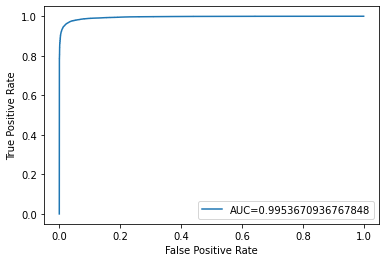
\includegraphics[width=1\linewidth]{Hinh_ve/LogisticRegression.png}
\caption{Biểu đồ đường cong đường cong ROC của mô hình LogisticRegression}
\label{fig:LRgression}
\end{figure}

\begin{figure}
\centering
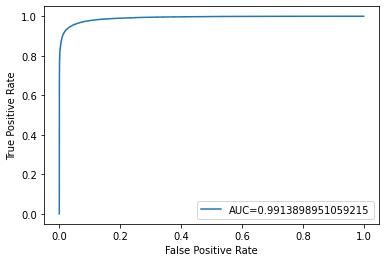
\includegraphics[width=1\linewidth]{Hinh_ve/MultinomialNB.png}
\caption{Biểu đồ đường cong ROC của mô hình Multinomial Naive Bayes}
\label{fig:MTilNB}
\end{figure}

\begin{figure}
\centering
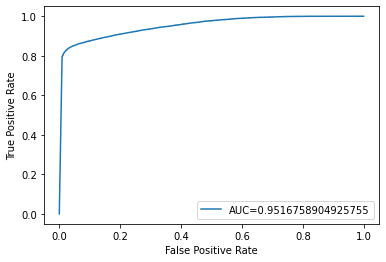
\includegraphics[width=1\linewidth]{Hinh_ve/BernoulliNB.png}
\caption{Biểu đồ đường cong ROC của mô hình Bernoulli Naive Bayes}
\label{fig:BerNB}
\end{figure}

\begin{figure}
\centering
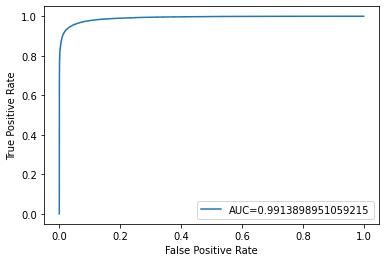
\includegraphics[width=1\linewidth]{Hinh_ve/ComplementNB.png}
\caption{Biểu đồ đường cong ROC của mô hình Complement Naive Bayes}
\label{fig:CompleteNB}
\end{figure}

\begin{figure}
\centering
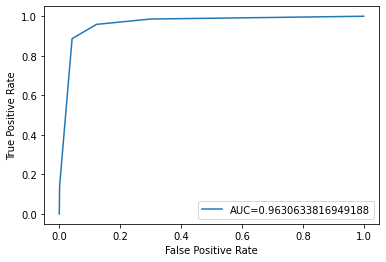
\includegraphics[width=1\linewidth]{Hinh_ve/KNeighborsClassifiepk4.png}
\caption{Biểu đồ đường cong ROC của mô hình KNeighborsClassifier với k = 4}
\label{fig:knnk4}
\end{figure}

\section{Kết quả tìm kiếm biến thể bằng biểu thức chính quy}
Áp dụng 47 biểu thức chính quy cho toàn bộ 124.850 bài báo trong bài báo được thu thập từ cơ sở dữ liệu Pubmed. Kết quả đã có 324.683 biến thể được tìm thấy trong thời gian chạy chương trình là 51 phút với CPU chạy đơn luồng.
Qua kiểm tra thủ công 10 bài báo ngẫu nhiên từ 124.850 bài báo trên. SỐ lượng biến thể tìm thấy là 29 biến thể. Trong đó các biến thể không tìm thấy là 41 biến thể. 



\subsection{Ví dụ về trường hợp biểu thức chính quy nhận diện đúng biến thể}
\begin{figure}
\centering
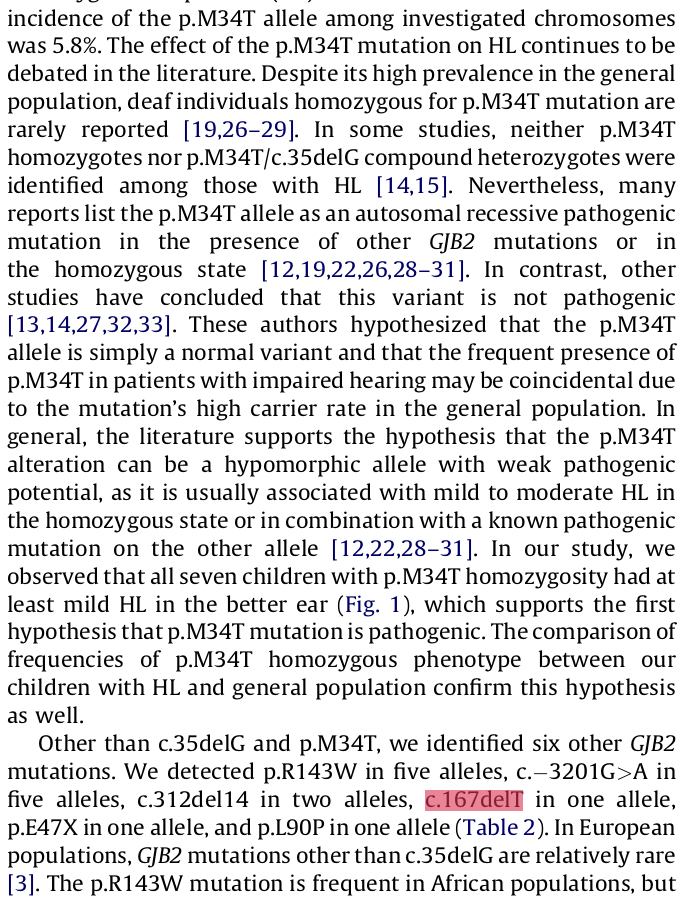
\includegraphics[width=1\linewidth]{Hinh_ve/PDFc167delTright.png}
\caption{Biến thể "c.167delT" được đề cập trong bài báo được phát hiện bởi biểu thức chính quy.}
\label{fig:PDFc167delTright}
\end{figure}

\begin{figure}
\centering
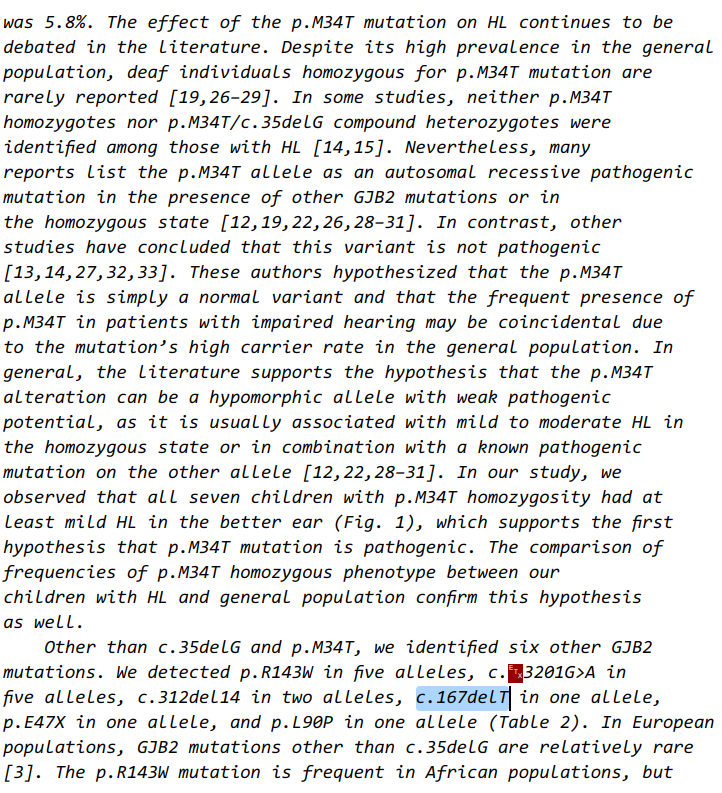
\includegraphics[width=1\linewidth]{Hinh_ve/TXTc167delTright.png}
\caption{Biến thể "c.167delT" được đề cập trong bài báo sau khi convert sang định dạng txt vẫn giữ nguyên định dạng. Biểu thức chính quy đã có thể tìm thấy biến thể này. Đây là biến thể mất đoạn xảy ra trên DNA tại vị trí 167 đã mất một nucleotides T. Cụ thể, "c." là đoạn DNA được sử dụng để tham chiếu, "167" là bị trí xảy ra đột biến, "del" là miêu tả đây là đột biến mất đoạn (Deletion Variant), "T" là nucleotides bị mất. Đoạn mô tả biến thể này sử dụng đúng theo tiêu chuẩn danh pháp HGVS.}
\label{fig:TXTc167delTright}
\end{figure}

Hình \ref{fig:PDFc167delTright} là định dạng ".pdf" của bài báo có tiêu đề ``Prevalence of c.35delG and p.M34T mutations in the GJB2 gene in Estonia``. Bài báo này được chuyển đổi sang dạng ".txt" vẫn giữ được cấu trúc, hình \ref{fig:TXTc167delTright}. Vì vậy, khi áp dụng biểu thức chính quy bên dưới, ta đã có thể tìm được biến thể này. 
\begin{center}{sep}c\.{pos}[, ]*?del(?!ins){space}?{origDna}(?!((ins)|{noDnas})){fs}?\end{center}

\subsection{Ví dụ về trường hợp biểu thức chính quy nhận diện sai và thiếu biến thể}
Hình \ref{fig:PDFwrong37doC} và hình  \ref{fig:TXTwrong37doC} là một ví dụ về nhận diện sai biến thể khi áp dụng biểu thức chính quy để tìm kiếm biến thể cho bài báo khoa học có tiêu đề ``Novel germline APC gene mutation in a large familial adenomatous polyposis kindred displaying variable phenotypes``, Bài báo truy cập trực tiếp tại địa chỉ ``https://pubmed.ncbi.nlm.nih.gov/7797123/``. Nguyên nhân nhận diện sai biến thể là do quá trình chuyển đổi từ định dạng pdf sang dạng text, có 1 ký tự bị chuyển đổi sai. Hình \ref{fig:PDFwrong37doC} là dạng đúng của ký tự 37 độ C. T , bị convert nhầm sang 370C. T ở hình \ref{fig:TXTwrong37doC}. Đoạn ký tự "370C. T" mô tả loại đột biến thay thế nucleotides C ở vị trí 370 thành nucleotides T. Tuy nhiên, biến thể này không được nhắc đến trong bài báo. 

\begin{figure}
\centering
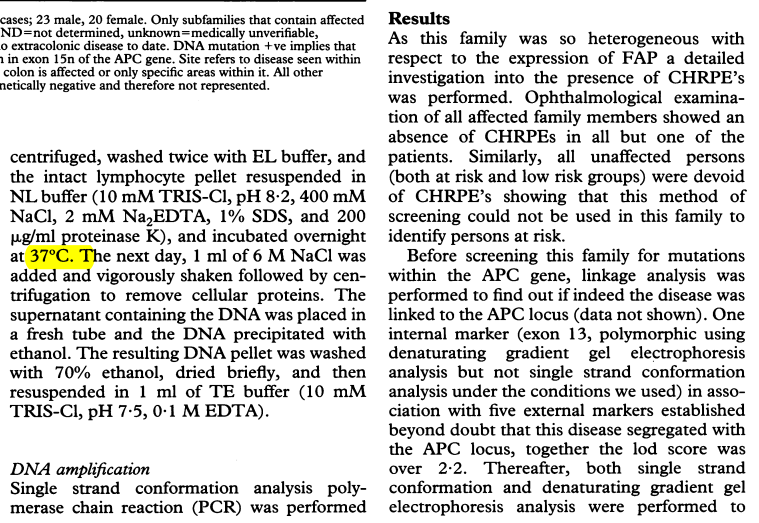
\includegraphics[width=1.0\linewidth]{Hinh_ve/PDFwrong37doC.png}
\caption{Một ví dụ về biểu thức chính quy nhận diện sai biến thể. Ký tự 37 độ C trong bài báo gốc ở định dạng pdf bị chuyển đổi sai thành 370C dẫn đến biến thể phát hiện được bị nhận thành 370C. T, đây là một đột biến thay thế nucleotides C ở vị trí 370 thành nucleotides T. Thực tế, trong bài báo không đề cập đến biến thể này}. 

Một ví dụ khác khi phát hiện biến thể trong bài báo có tiêu đề ``Characteristics of somatic mutation of the adenomatous polyposis coli gene in colorectal tumors``, bài báo này có thể truy cập trực tiếp tại địa chỉ: ``https://pubmed.ncbi.nlm.nih.gov/8187091/``. Có thể thấy rằng , định dạng văn bản gốc ở format pdf hình \ref{fig:PDFcttWrong} khi chuyển đổi sang format txt đã bị sai ký tự hình \ref{fig:TXTcttWrong}. Việc này cũng dẫn đến việc phát hiện sai biến thể và phát hiện thiếu biến thể.
\label{fig:PDFwrong37doC}
\end{figure}

\begin{figure}
\centering
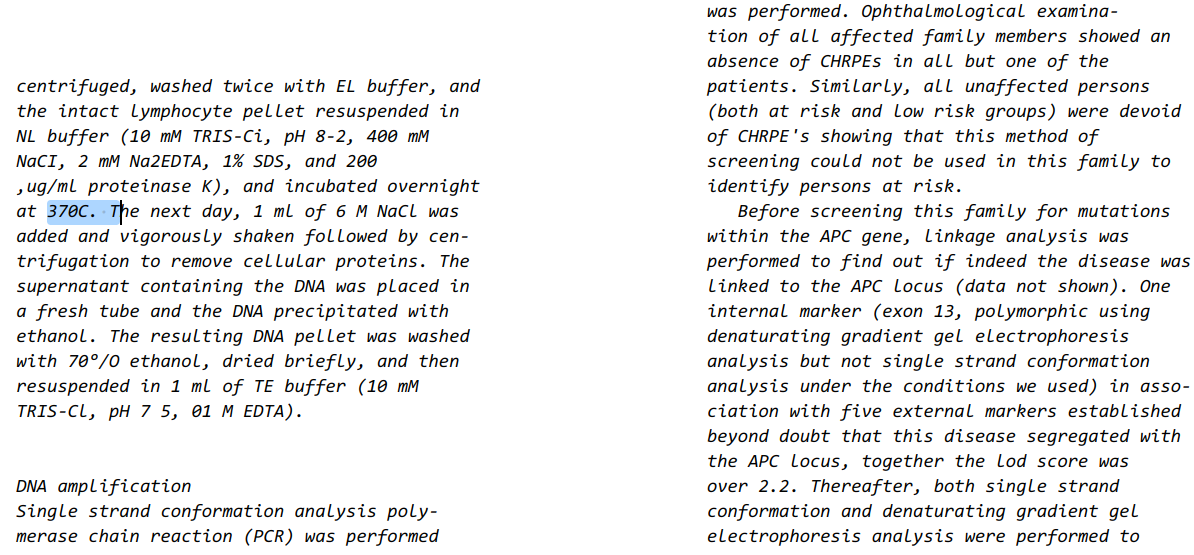
\includegraphics[width=1.05\linewidth]{Hinh_ve/TXTwrong37doC.png}
\caption{Ký tự 370 C trong bài báo gốc ở định dạng pdf bị chuyển đổi sai thành 370C dẫn đến biến thể phát hiện được bị nhận thành 370C. T, đây là một đột biến thay thế nucleotides C ở vị trí 370 thành nucleotides T. Thực tế, trong bài báo không đề cập đến biến thể này. }
\label{fig:TXTwrong37doC}
\end{figure}

\begin{figure}
\centering
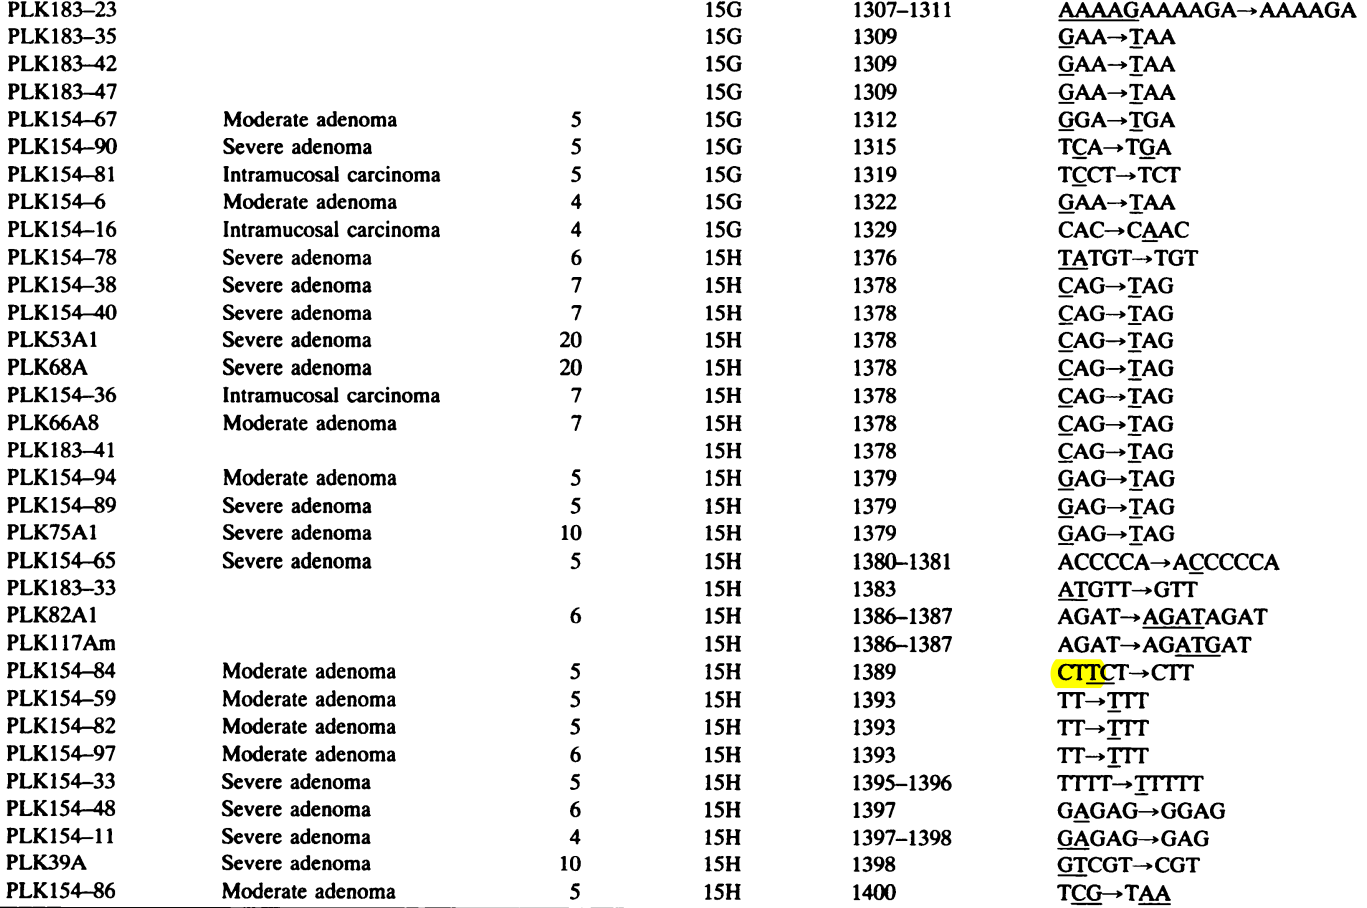
\includegraphics[width=1.0\linewidth]{Hinh_ve/PDFcttWrong.png}
\caption{Ký tự gốc trong bài báo là "CTTCT->CTT" bị chuyển đổi thành "C1TCi'—@CTT" trong hình \ref{fig:TXTcttWrong}, việc này dẫn điến việc nhận diện sai hoặc phát hiện không đầy đủ biến thể.}
\label{fig:PDFcttWrong}
\end{figure}

\begin{figure}
\centering
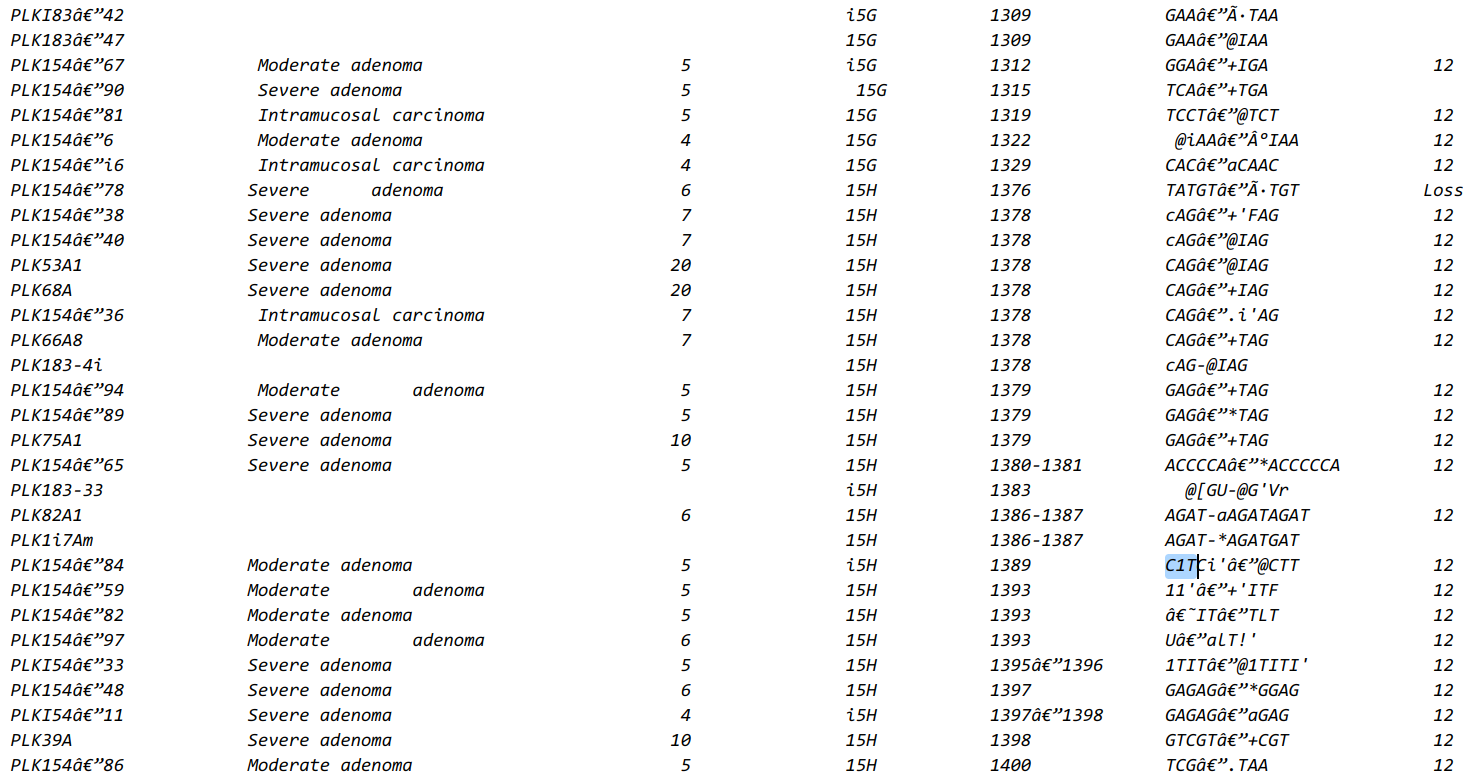
\includegraphics[width=1.0\linewidth]{Hinh_ve/TXTcttWrong.png}
\caption{Ký tự gốc trong bài báo là "CTTCT->CTT" hình \ref{fig:PDFcttWrong}  bị chuyển đổi thành "C1TCi'—@CTT", việc này dẫn điến việc nhận diện sai hoặc phát hiện không đầy đủ biến thể.}
\label{fig:TXTcttWrong}
\end{figure}


% Please add the following required packages to your document preamble:
% \usepackage{booktabs}
\begin{table}[]
\centering
\caption{Thống kê số lượng biến thể tìm thấy, biến thể không tìm thấy, và số lượng biến thể nhận diện sai bằng khi áp dụng biểu thức chính quy}
\label{tab:wrong_cvt}
\begin{tabular}{@{}|l|c|@{}}
\toprule
                        & \multicolumn{1}{l|}{Số lượng} \\ \midrule
Tổng số biến thể        & 70                            \\ \midrule
Biến thể tìm thấy       & 29                            \\ \midrule
Biến thể không tìm thấy & 41                            \\ \midrule
Biến thể nhận diện sai  & 31                            \\ \bottomrule
\end{tabular}
\end{table}

\end{document}